\chapter{Implementation \& Design}%
\label{implem}

\section{Problem Space}
Since the game is very complicated and can consist of many possible action spaces,
the majority of the experimentation focuses on the DeepMind mini-games
and simple small games in the \textbf{Simple64} map.

\subsection{Mini-games}

The mini-games consist of small, constrained challenges that represent
small parts of the full game of StarCraft II, allowing simple actions
in the game to be tested, as well as compared against a range of
published scores.

Every mini-game has a time limit, and the objective is to get the
highest score possible in the time frame.

These mini-games are:

\begin{itemize}
    \item MoveToBeacon: A simple map with a single marine (player controlled
        unit) and a beacon, which acts as a target to move to. The agent gets
        a point each time it reaches the beacon, at which point the beacon's
        location is reset.
    \item CollectMineralShards: A map with two marines and 20 mineral shards,
        which act as items to pick up. Once all are picked up, 20 more are
        placed on the map. To achieve an optimum score, the two marines must
        be controlled independently, which results in this map being
        harder than the MoveToBeacon map.
    \item FindAndDefeatZerglings: A map with three marines and 25 zerglings,
        which are an enemy unit. A point is achieved for each zergling that
        is defeated, and a point lost anytime a marine dies. This map
        is also the first to deal with the moving of the camera, as the previous
        two games had the entire state visible without moving the camera.
        Upon defeating the 25 zerglings, 25 more are added.
    \item DefeatRoaches: A map with nine marines and four roaches, which are a
        different enemy unit. This requires a more complex strategy to defeat,
        and also on defeating all four roaches, four more are spawned as well as 5
        more marines. This means the number of marines potentially grows
        throughout the game. However, a point is lost for any lost marines.
    \item DefeatZerglingsAndBanelings: A map with nine marines and six zerglings
        and four banelings. This again needs a different strategy and also gives
        extra marines upon defeating all the enemies.
    \item CollectMineralsAndGas: This map requires more strategy than the last.
        The map starts with 12 SCVs (which are gatherer units), a command centre
        (which is used to create additional units) and two types of collectable
        resources. The objective is to gather as many resources as possible, and
        also intelligently build more gathering units to increase the
        speed at which resources are gathered. An optimal strategy will also
        build an additional command centre.
    \item BuildMarines: This is the last and most complex map. The map starts
        with 12 SCVs, a command centre and eight resources to collect. The
        objective is to build as many marines as possible in the time limit.
        This requires the building of Supply Depots to store resources and
        barracks to build marines.
\end{itemize}

All of these mini-games have published scores for the many different
techniques as well as some baseline scores for human players and random
policies.

\subsection{The \textbf{Simple64} Map}

The \textbf{Simple64} map was also chosen to allow experimentation on
a straightforward version of the full game, where the challenge is
to beat the games AI, which is built using more traditional game AI
technology, and also can cheat at higher difficulties.

The map contains a single opponent and two starting bases. The agent is spawned
into one of the two areas randomly and starts out with the \textbf{SCV} units,
characters for building and mining. The initial stage begins with mining of
necessary of resources for progressing through the level by creating the required
buildings and training \textbf{Marines}, fighter characters. This needs the
agent to control the \textbf{SCV} and \textbf{Marine} units using complex three
action commands.

\section{StarCraft II API and SC2LE}

The SC2LE is an environment produced by DeepMind to provide a Python wrapper
for the StarCraft II API that is produced by Blizzard. This API allows both
information to be received from the game, as well as the sending on input to the
game. This is made even easier with the SC2LE, due to it serving up this API in
a language that fits directly with the Machine Learning libraries (Python, using
TensorFlow), as well as providing many different views of both the screen and
the mini-map, as can be seen in Figure~\ref{fig:sc2le}. In it, the main portion
of the screen shows the current screen and in the bottom left, the current
mini-map. The right-hand half of the screen has different views of both of the
screen and mini-map, showing different information in each.

\begin{figure}[h]
    \centering
    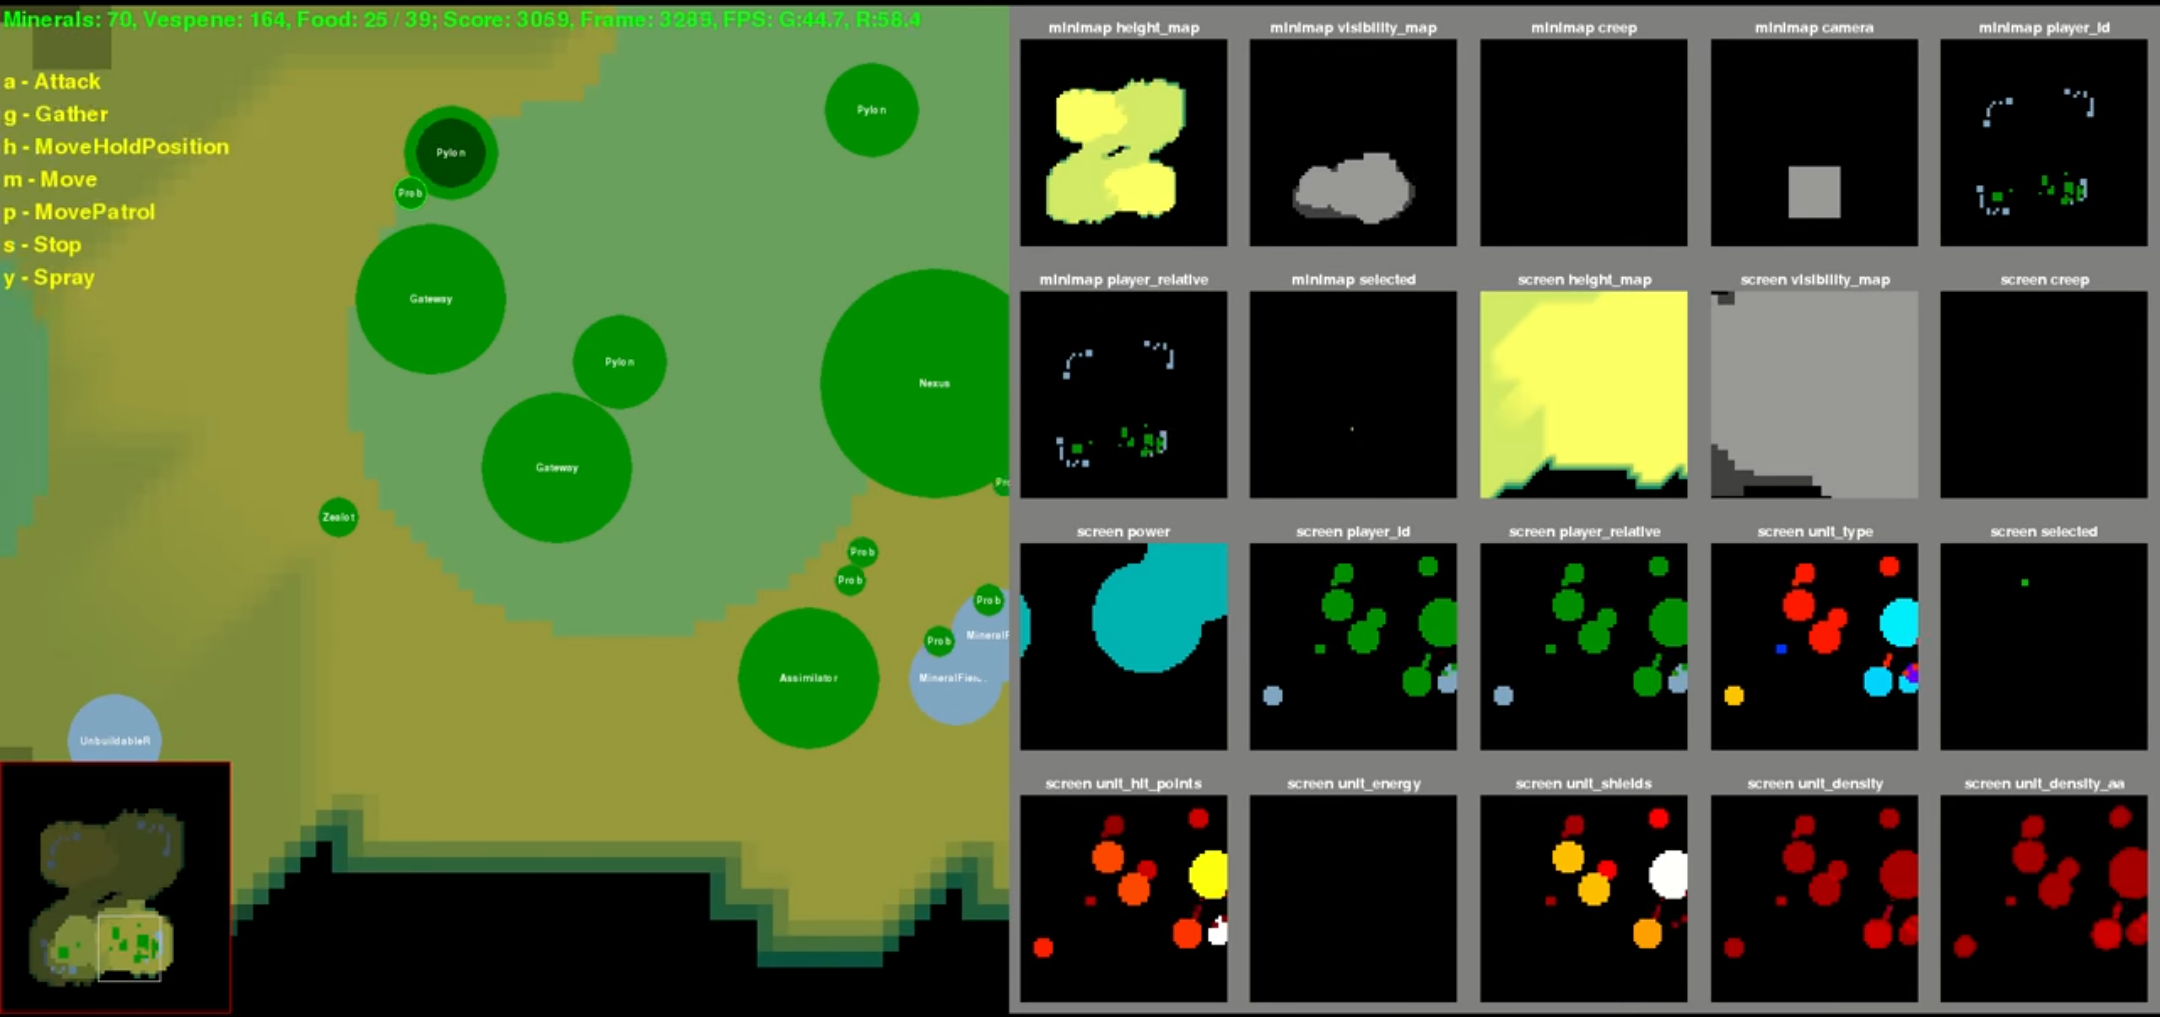
\includegraphics[width=1.0\textwidth]{pysc2}
    \caption{Example of the StarCraft II Learning Environment interface.}%
    \label{fig:sc2le}
\end{figure}

Using the SC2LE provides an easy interface to the game, such that game states
can be read, and input actions can be sent.  An agent takes an action based on
the given state, which in turn relies on how the information can be extracted
from the SC2LE\@.

To make the agent as close to a human player as possible, the API uses a grid to
represent most of the required information into a multiple array structure, where
each sub-array is concerned with a single aspect of the game. The arrays mostly
represent a grid-like structure, which can be treated as a simplified version of
the pixels that make up the game. Each sub-array is a column value with another
array to represent the row. This means that the agent would see information
about the world using a sampling of the available pixels.

An example would be the \texttt{screen} array which contains the columns and
sub-arrays that represent the row value. By indexing this array twice with
\texttt{`screen[x][y]'}, it is possible to get the value associated with grid
position \texttt{(x,y)}. The agent by default has a $64 \times 64$ grid view of
the current screen, and a second view of the same size of the mini-map.

The API implements an orthogonal projection to view the game world, as opposed
to how a human would see a perspective projection that is tilted to the side.
This is mainly due to the issue of overlapping units, where an agent would not
be able to distinguish them apart.

The API also provides access to the player mini-map. The mini-map provides:

\begin{itemize}
    \item The entire map view including unexplored areas, which are blacked out.
    \item All units and building in the game.
    \item Objects represented by an index for classification.
\end{itemize}

The classifications of the mini-map objects are:
\begin{enumerate}
    \item Background
    \item Agent's units
    \item Allied units
    \item Neutral units
    \item Hostile units
\end{enumerate}

The entire game state is accessed using the \texttt{observation} method provided
by the SC2LE\@. To access any information from the game, the user must index the
object with the relevant index since the \texttt{obs} variable is an array of
arrays with pertinent information. For example, to access the units of a given
type on the screen currently, the following code is used,
\texttt{obs.observation['screen'][UNITTYPE]}. The agent can see that a unit is
hidden through the mini-map but cannot identify the type of unit unless the
screen array is accessed for unit type information.

The screen array provides the following:

\begin{itemize}
    \item Powers of a selected unit
    \item The unit type
    \item Hit points of a selected unit
    \item Unit density (how many units are in a given area of the screen)
    \item More information on character abilities
\end{itemize}

For an action to be taken, a return call is made with the required action for
the step. This means that the action must be coded to select the relative unit
and return the coordinates for selecting the unit and issuing an action. This
makes most common actions in the game take multiple in-game steps, resulting in
even a common action such as movement being comprised of a selection step and
then an order to move.

There are two types of actions:

\begin{itemize}
    \item Queued: An action that will take place once the current
        action is finished.
    \item Immediate: Interrupts the current action being carried out and
        forces the character to begin the returned action.
\end{itemize}

Some actions require an extra parameter for position.
This makes the action space much more significant as the agent could choose any given
position to issue the action in a $64 \times 64$ grid.
So an action such as building a simple building would have $64 \times 64$
possible positions to represent the single action of building. However, this is
somewhat reduced due to some of the positions being invalid for a given action,
for example a building can not be built on top of an existing building.

\section{Development Choices}

As part of building an intelligent agent, or working with any form of deep
learning application, many parameters can be tuned that will alter the
performance of the network for a given task.

The most prominent challenge was identifying what information the agent would
need such that the input to the network was:

\begin{itemize}
    \item Useful in many states
    \item Critical to a given optimal decision
    \item Contextual
    \item Provides a baseline for what a unique state would look like
\end{itemize}

Once a state can be defined, the actions available to an agent will determine its
impact on the game world. The agent must be able to take actions that allow it to
transition between states with the ability to advance out of a loop created
by switching between the same states. This is what makes the choice of the input
state so crucial.

If given insufficient information, the agent could potentially make undesirable
choices due to not having enough information and performing the best
action that was visible.

This leads to what action in a given state is optimal and can the agent learn
whether the correct decision was made. The learning algorithm should allow an
agent to identify that remaining in a given loop is not the correct action and
that learning new actions could be the better outcome. Since this is using a
state action pair, the agent will not attempt to take any other actions that
have not been tested and defined to be the highest output.

\section{DeepQ Network}

The following section will focus on the Deep Neural Network that implements a
Q-Learning update function and policy evaluation.

\subsection{Network Architecture}

The network used for running the agent is comprised of the following layers:

\begin{enumerate}
    \item Input layer with 37 inputs for the state representation.
    \item First hidden layer with 50 nodes and a bias node.
    \item Second hidden layer with 40 nodes and a bias node.
    \item Third hidden layer with 25 nodes and a bias node.
    \item Output layer with 20 nodes (one for each possible action).
\end{enumerate}

The weights of each of the layers use a random normal distribution with a
standard deviation of 0.5 and a mean of 0. This allows the network to randomly
set the initial weights without the weights going beyond the range of -2 to +2.
If the weights are initialised to values that are greater than two, then the
network would overshoot in its calculations and assign incorrect values to the
weights with each update step. This then causes the network to tend to infinite
values since the TD error is always positive. The initial implementation used
random distributions without setting the standard deviation and caused the
network to overflow in values and tend to infinity. Since each layer will depend
on the previous multiplication and summation of the previous nodes when the
network was increased in size the values needed to be truncated to reduce the
weights from becoming too large.

The input may also need to be reduced due to the weight multiplication. In this
case, the input values were multiplied by 0.001 to minimise the overall
estimation of the network. This also requires the rewards to be reduced for the
TD Error evaluation.

\subsection{Exploration}

The agent uses an Epsilon-greedy algorithm for exploration. The algorithm works
by setting a value $\epsilon$ and taking the maximum value action for a given
state with a probability of $1-\epsilon$. Otherwise, the agent will take a random
action in that state. Using the Epsilon-greedy algorithm the agent can
learn the best action for a given state by randomly sampling different actions.
This helps the agent escape from the same loop of choosing the same action for a
given state.

The value of $\epsilon$ reduces with each time the agent takes a random action
so that the number of times the agent runs a random action is reduced. This is
known as Epsilon-decay function. The value of the decay is set before running
the network and is multiplied by the current $\epsilon$ every time a random
action is taken. The value of $\epsilon$ is therefore reduced with every
multiplication.

\begin{align}
    \epsilon = \epsilon \times decay
\end{align}

The initial value of $\epsilon$ is set to a high value such as 0.4. After a couple
of random actions taken the value of $\epsilon$ will reach a threshold value
(usually 0.1) and will no longer be multiplied by the decay factor. The agent
will then continue running with a fixed value of $\epsilon$ for the remainder of
the episodes. This allows the agent to start by testing more actions in
different states and eventually choosing the best action more often.

\subsection{Reward}

The agent can use a terminal reward system, where the final total reward is
given without live rewards, or live immediate reward system, where the agent is
given the reward during runtime. When using a terminal reward the agent will
receive the final reward without any immediate reward for what action in that
state may have achieved. Since the network implements a reward decay $\gamma$,
the agent will learn what pattern of actions and states helped to achieve that
final reward. This could lead to the problem of the agent over-fitting and
learning only a given pattern to take. However, the mini-games used for
evaluation will randomize the game state with every run. For example, the
MoveToBeacon map will randomly move the beacon to a different area of the map
every time. This makes it impossible for the agent to learn to move in a
specific pattern and achieve the same result. This does, however, take longer for
the agent to converge on the correct actions to take but will make the agent
increase the total reward at the end of each episode. If the agent is given an
immediate reward then the agent may try to achieve the same reward every time
without knowledge of how well it has performed overall. In some cases using a
live reward system may be favorable for the agent, but this would depend on the
task and requirement of the agent~\cite{shelton2001balancing}.

The agent's ability to learn the correct actions to take will depend on the
reward system. If the agent takes an action, the reward will define the value of
that taken action. This introduces the problem with live learning in a game that
runs in real-time. Since the game has actions that can take time to perform,
attacking for example, the agent will get the reward in the next few steps.
This means that the agent could take the correct action and then take another
action after it. The reward will go to the later action taken, but that is not
the action that was the correct one to take. For example, the agent decides to
attack an enemy unit and will receive a reward once the unit is dead, which
takes multiple attacks and is not instantaneous. The agent then takes the action
to build something, and at that given state the enemy unit was killed. This
would confuse the agent into assuming that the building action was the correct
action and not the attacking action. Using $\gamma$ can help rectify this issue.
The reward decay allows the agent to plan a couple of steps from the taken
action. The higher $\gamma$ is, the more it adds to the current state and action
value. Allowing the agent to associate higher values for the given state will
give better future outcomes, rather than the agent looking for the immediate
reward. Equation 3.5 shows $\gamma$ being multiplied by the next state's value
based on the best action to be taken next.

%TODO: Update the Equation 3.5 above to use \ref{} (by using \label on the
%equation). Just so its auto-generated since 3.5 is already wrong as far as I
%can tell.

\subsection{Learning}

The DeepQ network can be updated at the end of or during a game. Using an
offline network allows the agent to evaluate itself over all the choices made by
the agent during gameplay. The state, action, reward and next state are saved
into an array for updating the network once the episode is done. However, the
issue with offline learning is that the agent will not receive a reward for the
given action at the correct time and may require the agent be stopped for a
couple of steps.

\subsubsection{Off-Policy Learning}

%TODO: Fill in.

\subsubsection{Memory}

An array known as a ``memory'' is used for storing the state, action and rewards
from the episode. The memory array is then shuffled, which helps avoid learning
certain patterns or over-fitting. The memory array allows the agent to play
without losing any of the steps it took. Once the episode is finished, a
terminal state contains the final overall score of the agent.

\subsubsection{The Remember function}

The remember function is called at the end of every episode and triggers the
updating of the DeepQ network. The memory array is shuffled and sampled from one
array at a time. The array needs to be sampled in these single steps so that the
network can be run to test the next state prediction from the given state. The
function takes a single array that contains the state, action, reward and next
state from a single game step. The action is used to check the next state's
value. Once the network has been run on the next state, a value is returned
representing the next state's expected return. The loss function can then be
calculated using these two values.
